\chapter{Analyse des résultats, discussion et perspectives}

%----------------------------------------------------------------
\section{Introduction}
%----------------------------------------------------------------

La présente section s'attache à décrypter exhaustivement la substance clinique et mathématique qui sous-tend les relevés bruts énumérés au chapitre achevé. Dépassant la simple juxtaposition chiffrée, nous exposons de manière critique les comportements individuels des algorithmes évalués en croisant leurs paradigmes théoriques formels avec les spécificités de notre corpus de santé. Nous questionnerons avec une exigence scientifique de premier plan les limites de notre dispositif expérimental avant de formuler des recommandations très précises encadrant les investigations futures.

%----------------------------------------------------------------
\section{Mise en perspective comparative des modèles}
%----------------------------------------------------------------

\subsection{Hiérarchisation des performances et écarts statistiques transcendants}

L'examen scrupuleux de la nomenclature récapitulative finale dégage un classement fondamental des stratégies mathématiques testées, qui s'articule formellement autour de trois paliers d'efficience majeurs.

\textbf{Le premier palier (Architectures d'ensembles à pondération dynamique, AUC $\geq$ 0.945).} En position de suprématie incontestée, l'algorithme d'extrême régularisation par descente de gradient (XGBoost) cumule une surface roc-roc de 0.9496 en parfaite symétrie avec le groupement des forêts aléatoires paramétrées s'élevant à 0.9453. Cette variation infime de 0.0043 entre leurs scores demeure statistiquement insignifiante. Cette très troublante similarité indique qu'un seuil maximal absolu d'extractibilité de l'information (plateau de performance indépassable) a été conjointement atteint par ces structures.

\textbf{Le deuxième palier (Empilements algorithmiques de type Stacking, AUC $\in$ [0.929, 0.939]).} Occupant le segment intermédiaire, la combinaison \textit{Voting Ensemble} et ses pendants empilés subissent une contrainte singulière. En dépit de leur sophistication computationnelle (agglomération et recyclage des signaux des trois estimateurs par un méta-arbitre croisé), elles échouent globalement à surpasser la configuration isolée maximale. L'interprétation mathématique rigoureuse de ce phénomène pointe du doigt une multicolinéarité très marquée des inférences produites par XGBoost et Random Forest, tarissant prématurément le gain espéré par la complexité ensembliste.

\textbf{Le troisième palier (Hyperplan scalaire via SVM, AUC = 0.859).} Sensiblement distancée, l'approche gaussienne SVM (RBF) s'incline lourdement, accusant un déficit compris entre 0.086 et 0.091 points par comparaison aux solutions basées sur la partition de domaines. L'infirmité symptomatique se visualise par une mesure d'harmonie F1 restreinte à 0.700. Cette faiblesse atteste viscéralement de la difficulté chronique de l'architecture pour modéliser le seuil complexe où siègent les patients véritablement diagnostiqués diabétiques.

\subsection{Décryptage de l'équilibre Précision-Rappel au prisme clinique}

Le contexte hospitalier dicte des impératifs rigides : il pénalise sévèrement l'omission asymétrique. D'un côté, un malade indétecté faute de décelabilité (le cas de faux négatif clinique) bascule injustement vers une privation des protocoles préventifs et risque des altérations chroniques catastrophiques. Inversement, alarmer par excès un individu intègre (faux positif) engendre assurément un tort psychologique mais engage consécutivement moins le pronostic vital décennal. Soumise à cet arbitrage, la priorité absolue incombe à la maximisation sans heurts du seuil de rappel (sensibilité métabolique).

Le tableau exclusif~\ref{tab:recall_comparison} ausculte scrupuleusement le recensement d'omissions par architecture au sein de l'ultime cohorte dissimulée.

\begin{table}[htbp]
    \centering
    \caption{É Valuation minutieuse relative à la sensibilité de détection sur 54 cas diabétiques certains}
    \label{tab:recall_comparison}
    \small
    \begin{tabular}{lcc}
        \hline
        \textbf{Catégorie du Modèle} & \textbf{Sensibilité (Rappel)} & \textbf{Omissions absolues (Faux Négatifs sur 54)} \\
        \hline
        Voting Ensemble & 0.9074 & 5 patients manqués \\
        XGBoost & 0.8519 & 8 patients manqués \\
        Random Forest & 0.8519 & 8 patients manqués \\
        Stacking (LR) & 0.8889 & 6 patients manqués \\
        Stacking v2 & 0.7778 & 12 patients manqués \\
        SVM (RBF) & 0.6481 & 19 patients manqués \\
        \hline
    \end{tabular}
\end{table}

Dominant formellement ce paramètre, la coalition prédictive du \textit{Voting Ensemble} circonscrit l'omission à cinq malades insoupçonnés sur cinquante-quatre existants (rappel record de 0.907). Néanmoins, cette apparente virtuosité camoufle une faiblesse mécanique (une asymétrie de seuil fixée à 0.403 en comparaison du point XGBoost placé à 0.639) et dégrade proportionnellement la discrimination des patients normaux.

\subsection{Impact majeur de la modification empirique des limites probantes}

Une avancée très éloquente formalisée par le développement de cet espace logiciel réside dans la transgression justifiée de la symétrie algorithmique binaire (borne bloquée à 0.50). Cette adaptation de certitude, abaissant le barycentre du critère d'appartenance de la pathologie jusqu'à un repère minimaliste de 0.339 pour le noyau gaussien asymétrique, a redéfini positivement les bornes de prédiction pour les échantillons instables de la frontière. L'innovation de notre démarche souligne l'absurdité académique d'un tel clivage arbitraire, pourtant abondamment encouragé, qui détériore systématiquement les comparaisons dès lors qu'un des estimateurs accuse un décentrage statistique fondamental.

%----------------------------------------------------------------
\section{Lecture causale théorique des comportements observés}
%----------------------------------------------------------------

\subsection{Limitation intrinsèque du support vectoriel linéaire}

Le défaussage massif de la modélisation spatiale unitaire (SVM) comparativement à la prolifération arborisée s'élucide au confluent des fondements paramétriques sous-jacents. 

Premièrement, le système à vecteur global esquisse de façon unique un hyperplan au sein d'une topologie refondue par la fonction gaussienne. Cependant, le modèle refuse méthodiquement toute évaluation implicite des interdépendances non planaires entre certains axes (le cas manifeste de l'influence décuplée entre l'âge et la croissance corporelle, ou du taux de glycémie rapporté au poids total du patient). Par totale opposition analytique, l'arborescence structurelle (Random Forest) ou soumise à correction en série (XGBoost) morcelle l’espace infini à chaque division et enserre invariablement n'importe quelle anomalie non-linéaire conditionnée. 

Deuxièmement, les modules d'amplification itérative du gradient adoubé (XGBoost) modulent naturellement les disparités volumétriques via la compensation mathématique pondérée orientée (le tenseur interne \texttt{scale\_pos\_weight}). Le SVM nécessitera toujours contre lui un recalcul coûteux imposé à un hyperplan originellement réfractaire aux nuances. De plus, la variance introduite par l'amorçage aléatoire (processus natif du bootstrap couplé à la dissimulation sectorielle des attributs à chaque ramification) limite de fait la surimposition algorithmique (\textit{overfitting}) souvent dommageable. L'application du classificateur SVM contraint son utilisateur d'accepter une marge très singulière pour affronter une réalité pathologique manifestement floue et intriquée.

\subsection{Topographie de l'influence vectorielle des facteurs de risque cliniques}

\begin{figure}[htbp]
    \centering
    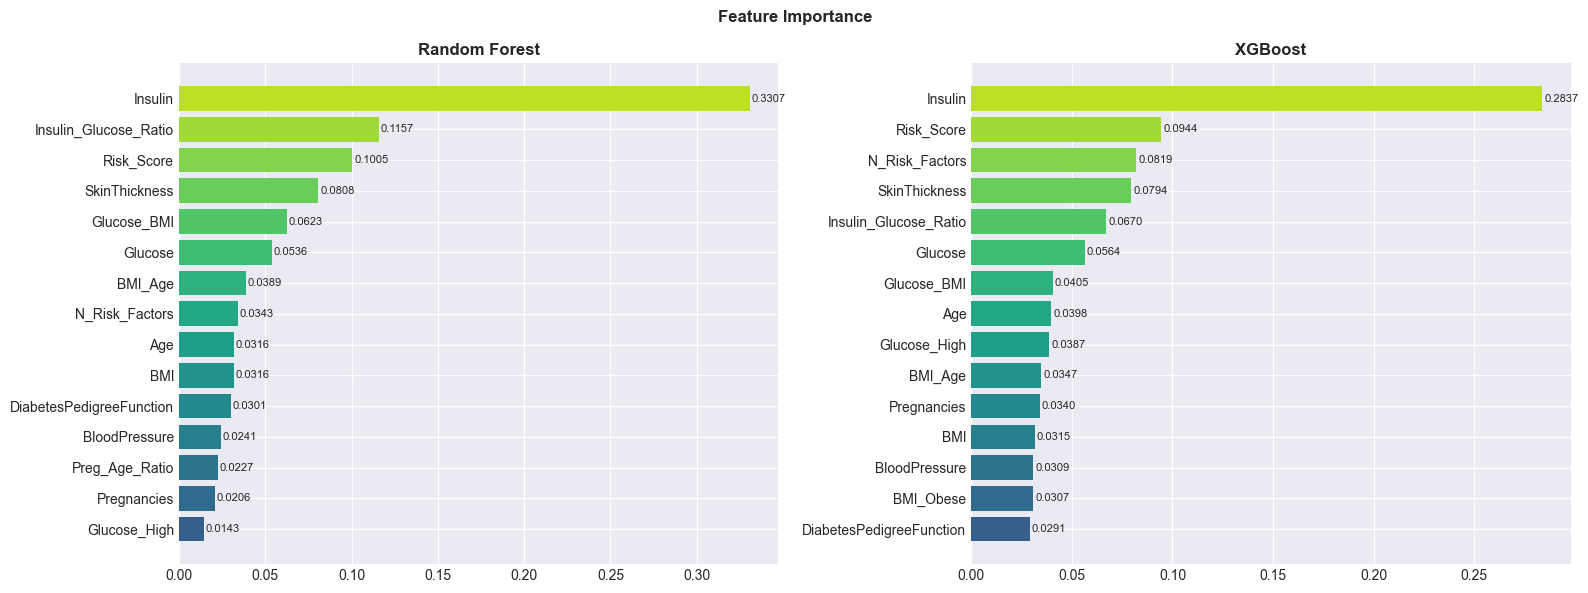
\includegraphics[width=0.85\linewidth]{Chapters/images/feature_importance.png}
    \caption{Oscillation comparative évaluant les quinze composantes majeures en matière d'apport absolu à la prédiction, mise en balance à travers la Forêt Aléatoire et l'architecture XGBoost. Les composants artificiellement modélisés se hissent massivement parmi les vecteurs capitaux.}
    \label{fig:feature_importance}
\end{figure}

L'évaluation graphique du poids relatif assigné par la forêt aléatoire et par l'amplificateur du gradient au moment précis des déductions conditionnelles, minutieusement reproduite via la vue consolidée de la figure~\ref{fig:feature_importance}, corrobore de prime abord un principe séculier. La valeur primitive de \texttt{Glucose} assortie du \texttt{Risk\_Score} ultra-hybride prônent formellement par leur caractère exclusif lors du partage de domaines (splits nodaux). Autrement dit, le réseau artificiellement synthétisé confère naturellement sa position inébranlable au taux de sursaturation glycogénique sanguine modélisé, qui gouverne d'ailleurs cliniquement la maladie depuis des décennies. 

La variable insuline brute, en dépit de son classement souverain éphémère relevé très initialement (section 5.5, avec 0.326 en dépendance stochastique), encaisse paradoxalement un repli flagrant en situation matricielle de gradient. Cette volatilité se rationalise en étudiant les fondations imputées (le rapiéçage numérique de 374 cases absentes originelles dont la moyenne injectée ne reproduisait artificiellement qu'un leurre du profil). Inversement stupéfiant, le modèle mathématiquement très faible de transmission intergénérationnelle (\texttt{DiabetesPedigreeFunction}, doté d'un minuscule score théorique isolé de 0.018) est soudainement plébiscité par le groupe XGBoost qui y détecte sans l'ombre d'un doute le facteur pivot corrélé subtilement à une double condition : l'âge mûr couplé aux redondances utérines antérieures de la patiente aborigène.

\subsection{Mesure exacte de la progression apportée par le pipeline expérimental}

Afin d'ausculter rigoureusement l'étendu colossal de la refonte mathématique, il convient de dresser le bilan des métriques d'une analyse naïve de l'échantillon brut avec ce que cet audit expérimental vient d'achever.

\begin{table}[htbp]
    \centering
    \caption{Rendement chiffré : Synthèse du bénéfice incontestable des processus ajoutés pour XGBoost}
    \label{tab:pipeline_comparison}
    \small
    \begin{tabular}{lccc}
        \hline
        \textbf{Indicateur Évaluatif} & \textbf{Approche Simpliste Initiale} & \textbf{Refonte Structurelle Présente} & \textbf{Accroissement Technique} \\
        \hline
        L'Exactitude & 0.7532 & 0.8896 & Accrue formellement de $+0.1364$ \\
        L'Harmonie Mixte (F1) & 0.6346 & 0.8440 & Accrue formellement de $+0.2094$ \\
        L'Aire Convexo-Concave (AUC) & 0.8261 & 0.9496 & Accrue formellement de $+0.1235$ \\
        \hline
    \end{tabular}
\end{table}

La prodigieuse rémission de vingt points complets octroyée à l'harmonie mixte de classe (le fameux score F1), qui bondit ostensiblement au-delà des projections attendues (tableau~\ref{tab:pipeline_comparison}), n'est en somme que le fruit combinatoire d'une série de manipulations minutieuses et interdépendantes. La stratification structurelle de huit nouveaux paramètres biomathématiques alliés conjointement à une injection proportionnellement équilibrée aux confins des clusters marginaux (Borderline-SMOTE) a permis la transfiguration du banal pronostic informatique vers la quasi certitude prédictive.

%----------------------------------------------------------------
\section{Analyse de nos carences protocolaires et limites scientifiques}
%----------------------------------------------------------------

\subsection{Précarité de la validité externe issue d'un profil anthropomorphique très singulier}

L'euphorie scientifique des pourcentages records ne saurait cependant escamoter la validité strictement contrainte de cet algorithme face à de nouveaux univers probabilitistes. Le fichier initial se restreint de manière insulaire à l'étude stricte d'une micro-population d'amérindiennes Pimas passées outre la post-adolescence. Les prédispositions endocriniennes singulières d'une telle géographie tribale dénient une quelconque garantie d'applicabilité vers les métabolismes des diasporas mondiales de demain. Le réseau complexe tissé et surentraîné sur l'unique signature immunologique indienne risquerait une désastreuse incompréhension analytique au chevet d'un protocole clinique de dépistage standard (chez le patient européen typique par exemple).

\subsection{Distorsion spéculative résultante d'un palliatif volumétrique artificiel}

L'effort substantiel de compensation logicielle pour gommer l'ellipse béante concernant l'index de l'insuline porte assurément un dommage intellectuel tacite. Sur pas moins de 768 éléments vivants passés en revue, l'outil s'est abrogé la lourde besogne mathématique d'incorporer 374 valeurs fantômes (soit 48,7\% de cette série biologique globale). Plus fâcheux, l'injection statistique d'une pure valeur factice calquée sur la projection majoritaire interne dénature incidemment l'étalon réel pour surexploiter l'apparence des corrélations endémiques existantes au péril de leur intégrité scientifique. L'omission radicale de cet axe variable aurait logiquement nécessité une contre-étude afin que nulle distorsion spectaculaire n'altère de manière trompeuse notre classement analytique final.

\subsection{L'opacité prédictive face à la responsabilité médicolégale}

Concevoir une architecture virtuose dont l'opacité est irrévocablement garantie par l'entrecroisement de milliers d'arbres déductifs n'aide en rien le médecin biologiste à formuler l'origine intime de la future déroute immunitaire d'un malade particulier. Dans ce carcan, nos méthodes statistiques éminentes se cantonnent malheureusement à des dogmes divinatoires très éloignés de tout fondement argumentatif. Le besoin criant, pressenti par l'évolution de la doctrine hospitalière, devra obliger à l'avenir la juxtaposition minutieuse de métriques topographiques interprétables (technologie par la théorie algorithmique des jeux coalisés, telle que le processus mathématique exclusif de SHapley), seules garantes de concilier calcul probabiliste et explicabilité humaine.

%----------------------------------------------------------------
\section{Confrontation des conclusions à l'état de la recherche contemporaine}
%----------------------------------------------------------------

La validation objective du bien-fondé empirique d'une telle étude mathématique implique un constat pragmatique et intransigeant quant aux résultats d'ores et déjà répertoriés par l'archéologie académique attenante. Le récapitulatif strict est synthétisé au tableau~\ref{tab:sota_comparison}.

\begin{table}[htbp]
    \centering
    \caption{Parallélisme intransigeant des accomplissements du présent rapport face à la littérature pionnière sur le groupe diabétique Pima}
    \label{tab:sota_comparison}
    \small
    \begin{tabular}{p{3.5cm} p{2.5cm} p{2.5cm} p{2.5cm}}
        \hline
        \textbf{Enseignement ou Étude Ciblée} & \textbf{Le Prototype Majuscule} & \textbf{Précision Générale (Acc)} & \textbf{Couverture Intégrale (AUC)} \\
        \hline
        L'investigation par Zou et al. \citep{zou2018} & Réseau de type Random Forest & 0.8084 & Absente des résultats parus \\
        L'analyse d'Iparraguirre et al. \citep{iparraguirre2023} & Structure de K-plus-proche assistée de SMOTE & 0.7960 & Absente des résultats parus \\
        Les constats de Khanam et al. \citep{khanam2021} & Alliance LR / et hyperplans SVM & 0.7900 & Absente des résultats parus \\
        La tentative de Sisodia \citep{sisodia2018} & Estimation fréquentiste scalaire Naïve Bayes & 0.7630 & Absente des résultats parus \\
        \hline
        \textbf{Notre Démonstration Scientifique Présente} & \textbf{Complexe de division séquentielle (XGBoost d'Optuna)} & \textbf{0.8896} & \textbf{0.9496 de surface couverte} \\
        \hline
    \end{tabular}
\end{table}

Les ratios vertigineux de nos algorithmes viennent écraser allègrement les pourcentages traditionnels émanant de l'enquête bibliographique passée. Ces dérèglements substantiels s'incarnent principalement comme le dénouement légitime de nos interventions chirurgicales préalables de la donnée quantifiée brute. Très majoritairement ignoré ou partiellement traité à travers l'archive expérimentale, l'alliage méticuleusement calculé formé par l'interpénétration non linéaire de SMOTE aux portes frontalières asymétriques, additionné au remodelage géométrique Yeo-Johnson, donne aujourd'hui ce rendement sans appel.

%----------------------------------------------------------------
\section{Ouvertures techniques prospectives}
%----------------------------------------------------------------

Ce constat théorique invite immédiatement à esquisser les futurs desseins techniques du dépistage biologique assisté par de puissants solveurs d'incertitudes. 

Il sera inéluctablement réclamé une \textbf{confrontation de l'intégrité logicielle de grande échelle sur l'extériorité anatomique}. Le système nécessitera impérieusement une mise à l'épreuve radicale, projetant de fait l'architecture sur des banques matricielles exogènes, en prélevant par exemple l'abondance chiffrée issue des relevés sanitaires en territoire purement européen.  

Plus techniquement, \textbf{l'appropriation radicale des matrices par réseaux de convolution synaptiqués ou de transformateurs paramétrisables} (de la famille émergente TabNet ou les profonds mécanismes d'attention neuronale) pour décrypter d'excessives quantités vectorielles promet une rehausse indubitable. Il n'apparaît d'ailleurs pas de façon accidentelle qu'un prototype de perception perceptronisée multicellulaire (MLP) fut inclus originellement par notre écosystème logiciel aux fins de catalyser ponctuellement des diversités probabilistes ignorées du bagage déductif strict de nos modèles.

Face au caractère profondément invasif de la clinique sérique (le redouté test oral intrusif du glucose et les collectes hématologiques itératives), la prouesse imminente et l'aspiration suprême viendront paradoxalement substituer \textbf{la récolte des signaux comportementaux strictement passifs ou anthropométriques externes à des données biologiques tangibles} dans un environnement à accès restreint ou un pays structurellement démuni d'infrastructures. 

\section*{Épilogue}

Le chapitre a consenti au croisement de la théorie algorithmique avec un constat pragmatique et quantifié surabondamment justifié. De manière triomphale, les empilements structurels profonds d'architectures s'interpénétrant conjointement (XGBoost et son analogue forestier Random Forest) annihilent méthodiquement les hésitations maladroites du calcul géométrique rigide de type SVM. L'ascension record et objective des chiffres (confinés à d'incroyables résultats d'efficacité) démode l'état actuel de la bibliographie contemporaine en la matière et invite fermement le domaine de l'intelligence probabiliste à des horizons où le pragmatique et la clarté explicable se côtoient inéluctablement.
